\Variant{12.10.2024 (2-smena)}
\QQ{1}{Natural $a$ va $b$ sonlar uçun $a\cdot b=24$ tenglik bajarilsa, $a+2b-1$ ning eng katta qiymatini toping.
\Opts{$25$}{$30$}{$10$}{$48$}}
\QQ{2}{Hisoblang:
\[81^{0{,}75}\cdot32^{-\frac25}-27^{0{,}(3)}\cdot16^{-0{,}5}+256^{\frac12}\]
\Opts{$1$}{$22$}{$30$}{$10$}}
\QQ{3}{A şahardan B şaharga 1-avtomobil özgarmas $120$ km/h tezlik bilan, $10$ daqiqadan söng 2-avtomobil $150$ km/h tezlik bilan yölga çiqdi. Ular B şaharga bir vaqtda yetib keldi. A va B şaharlar orasidagi masofani toping.
\Opts{$100$}{$120$}{$50$}{$60$}}
\QQ{4}{Töğri törtburçakning eni $25\%$ ga, böyi $20\%$ ga ortgan bölsa, yuzi neça foizga ortgan?
\Opts{$45$}{$50$}{$60$}{$5$}}
\QQ{5}{Ifodani soddalaştiring:
\[\frac{77^{2m}}{7^{m-1}\cdot11^m\cdot7^m\cdot11^{m+1}}\]
\Opts{$\dfrac{77}5$}{$\dfrac7{11}$}{$\dfrac{11}7$}{$1$}}
\QQ{6}{Hisoblang:
\[\left(\frac{\sqrt6+2\sqrt3-\sqrt2-2}{\sqrt6+\sqrt3-\sqrt2-1}\right)^2\]
\Opts{$2$}{$\sqrt2-1$}{$\sqrt2+1$}{$1$}}
\QQ{7}{Hisoblang:
\[\frac3{2\sqrt[3]2+2\sqrt[3]4}-\frac3{2\sqrt[3]2-2\sqrt[3]4}+\sqrt[3]4\]
\Opts{$\sqrt[3]4+1$}{$\sqrt[3]{16}+1$}{$\left(\sqrt[3]4+1\right)^2$}{$-\left(\sqrt[3]4+1\right)^2$}}
\QQ{8}{Tengsizlikni qanoatlantiruvçi natural sonlar köpaytmasini toping:
\[\frac{x^2-6x+8}{x-1}-\frac{x-4}{x^2-3x+2}\le0\]
\Opts{$6$}{$3$}{$12$}{$4$}}
\QQ{9}{Arifmetik progressiyada $a_{11}=40$, $a_{31}=-20$ bölsa, $\dfrac{a_{101}}{a_{91}}$ ni toping.
\Opts{$\dfrac3{20}$}{$\dfrac{20}{23}$}{$1\dfrac3{20}$}{$\dfrac{17}{23}$}}
\QQ{10}{Geometrik progressiyaning dastlabki uçta hadi $\log_2x-2$; \ $\log_2(2x)$; \ $\log_2(4x)+5$ ga teng bölsa, $x$ ni toping.
\Opts{$16$}{$64$}{$4$}{$32$}}
\QQ{11}{$x=3$, $y=\sqrt3$ bölsa,
\[\left(x^3+xy^2+\frac{xy\left(x^2+y^2\right)}{x-y}\right)\cdot\left(\frac{xy}{x+y}-x\right):\frac{x^2\left(x^2+y^2\right)}{x^2-y^2}\]
ni hisoblang.
\Opts{$-9$}{$9$}{$3$}{$-\sqrt3$}}
\QQ{12}{Tengsizlikni yeçing:
\[\frac{25x-5}{|x-1|}>0\]
\Opts{$\left(-\infty;\,\dfrac15\right)$}{$\left(\dfrac15;\,1\right)\cup(1;\,\infty)$}{$\left(\dfrac15;\,\infty\right)$}{$(1;\,\infty)$}}
\QQ{13}{$7x^2-6x+1=0$ tenglamaning ildizlari $x_1$ va $x_2$ bölsa, ildizlari $\dfrac1{x_1^2}$ va $\dfrac1{x_2^2}$ bölgan keltirilgan kvadrat tenglamaning koeffitsiyentlari yiğindisini toping.
\Opts{$70$}{$29$}{$28$}{$68$}}
\QQ{14}{Tengsizlikni neçta butun son qanoatlantiradi?
\[7^{3x}+1\le7^{x-1}\cdot\left(55\cdot7^x-41\right)\]
\Opts{$1$}{Çeksiz köp}{$2$}{$5$}}
\QQ{15}{Ifodani soddalaştiring:
\[\frac{(\sin x-\cos x)^2}{\sin^2\left(\frac\pi4-x\right)}\]
\Opts{$2$}{$\dfrac{1-\sin2x}{1+\sin2x}$}{$\dfrac{2(1-\sin2x)}{1-\cos2x}$}{$1$}}
\QQ{16}{Tenglamaning ildizlar köpaytmasini toping:
\[\log_2^2x+(x-1)\log_2x+2x=6\]
\Opts{$\dfrac12$}{$4$}{$2$}{$\dfrac14$}}
\QQ{17}{$(x+1)(x+4)(x-2)(x+7)=19$ tenglamaning ildizlar yiğindisini toping.
\Opts{$-10$}{$-13$}{$-17$}{$-19$}}
\QQ{18}{Tenglama $\left[-\dfrac\pi2;\,\pi\right]$ oraliqda neçta yeçimga ega?
\[\cos3x-\sin2x=0\]
\Opts{$5$}{$6$}{$7$}{$8$}}
\QQ{19}{Agar $|x-5|\le3$ bölsa, $9\left(\dfrac12x-2\right)^2-\left(\dfrac12x-2\right)^4$ ifodaning eng katta qiymatini toping.
\Opts{$18$}{$20$}{$22$}{$81$}}
\QQ{20}{Agar $\dfrac xy=2023$ bölsa, $\dfrac{x^2-xy}{xy}=\ ?$
\Opts{$2022$}{$2023$}{$2024$}{$2012$}}
\QQ{21}{Integralni hisoblang:
\[\int\frac{2x^2+1}{x^4+x^2}\,dx\]
\Opts{$-\dfrac1{x^2+1}+\arctg(x+1)+C$}{$\dfrac1x+\arctg x+C$}{$-\dfrac1x+\arctg x+C$}{$x+\arctg x+C$}}
\QQ{22}{Quyidagi funksiyalardan neçtasi juft funksiya?
\[y_1=\sin^2x+\sqrt[3]{|x|};\quad y_2=\cos^2x+\sqrt[3]{x^2};\quad y_3=\tg^3x+\sqrt{|x|};\quad y_4=\ctg^4x+\sqrt[4]{|x|^3}\]
\Opts{$1$}{$2$}{$3$}{$4$}}
\QQ{23}{Markazi $(4;\,3)$ nuqtada bölgan aylana $Oy$ öqiga urinadi. Şu aylana radiusini toping.
\Opts{$3$}{$4$}{$5$}{$7$}}
\QQ{24}{$ABC$ uçburçakning yuzi $60$ ga teng. $\overrightarrow{BF}=\dfrac12\overrightarrow{AB}$, $\overrightarrow{BE}=\dfrac12\overrightarrow{BC}$ bölsa, $BEF$ uçburçak yuzini toping.
\Opts{$15$}{$20$}{$30$}{$45$}}
\QQ{25}{$y=\left|x^2-4x+3\right|$ funksiyaning $[2;\,4]$ oraliqda eng katta va eng kiçik qiymatlari yiğindisini toping.
\Opts{$5$}{$4$}{$3$}{$12$}}
\QQ{26}{$x$ ning qabul qilişi mumkin bölgan eng katta natural qiymatini toping.
\qfig{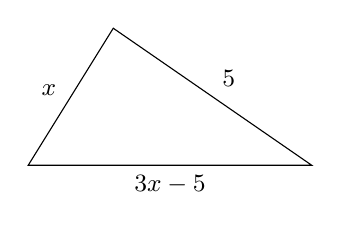
\begin{tikzpicture}[scale=0.6,font=\small]
\draw (0,0)--(6,0)--(1.8,2.9)--cycle;
\node[left] at (0.8,1.6) {$x$}; \node[above right] at (3.9,1.45) {$5$}; \node[below] at (3,0) {$3x-5$};
\end{tikzpicture}}
\Opts{$4$}{$5$}{$2$}{$3$}}
\QQ{27}{$EFLM$, $FGNL$, $MNKA$, $ABCD$ — kvadratlar berilgan. Agar $EM=5$ bölsa, $FNC$ uçburçak yuzini toping.
\qfig{\begin{tikzpicture}[scale=0.13,font=\small]
\coordinate (E) at (0,0); \coordinate (M) at (5,0); \coordinate (A) at (15,0); \coordinate (D) at (35,0); \coordinate (F) at (0,5); \coordinate (L) at (5,5); \coordinate (G) at (0,10); \coordinate (N) at (5,10); \coordinate (K) at (15,10); \coordinate (B) at (15,20); \coordinate (C) at (35,20);
\fill[qfill] (F)--(N)--(C)--cycle;
\draw (E)--(D)--(C)--(B)--(A); \draw (E)--(G)--(N)--(K); \draw (F)--(L); \draw (M)--(N); \draw (F)--(N)--(C)--cycle;
\draw (14.3,5)--(15.7,5); \draw (14.3,15)--(15.7,15);
\node[below] at (E) {$E$}; \node[below] at (M) {$M$}; \node[below] at (A) {$A$}; \node[below] at (D) {$D$}; \node[left] at (F) {$F$}; \node[below right] at (L) {$L$}; \node[left] at (G) {$G$}; \node[above] at (N) {$N$}; \node[below right] at (K) {$K$}; \node[above] at (B) {$B$}; \node[above right] at (C) {$C$};
\node[below] at (2.5,0) {$5$};
\end{tikzpicture}}
\Opts{$50$}{$100$}{$40$}{$45$}}
\QQ{28}{$ABCDEF$ muntazam oltiburçakning yuzi $36$ ga teng. Böyalgan $BDF$ uçburçakning yuzini toping.
\qfig{\begin{tikzpicture}[scale=1.1,font=\small]
\foreach \n/\a in {A/180,B/120,C/60,D/0,E/-60,F/-120} {\coordinate (\n) at (\a:1); \node at (\a:1.2) {$\n$};}
\fill[qfill] (B)--(D)--(F)--cycle;
\draw (A)--(B)--(C)--(D)--(E)--(F)--cycle; \draw (B)--(D)--(F)--cycle;
\end{tikzpicture}}
\Opts{$16$}{$18$}{$20$}{$24$}}
\QQ{29}{$CF=6$, $CG=7$, $GE=5$ va $ED=6$ bölsa, $FG$ kesma uzunligini toping.
\qfig{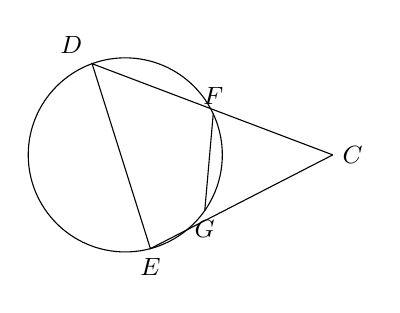
\begin{tikzpicture}[scale=0.85,font=\small]
\coordinate (O) at (0,0); \coordinate (D) at (110:1.45); \coordinate (E) at (-75:1.45); \coordinate (F) at (25:1.45); \coordinate (G) at (-35:1.45); \coordinate (C) at (3.1,0);
\draw (O) circle (1.45); \draw (C)--(D)--(E)--(C); \draw (F)--(G);
\node[above left] at (D) {$D$}; \node[below] at (E) {$E$}; \node[above] at (F) {$F$}; \node[below] at (G) {$G$}; \node[right] at (C) {$C$};
\end{tikzpicture}}
\Opts{$6$}{$4$}{$2$}{$3$}}
\QQ{30}{Tekislikka ikkita oğma va perpendikulyar tuşirilgan. Agar $AD=4$, $\angle ABD=45^\circ$, $\angle BAC=30^\circ$, $\angle ACD=30^\circ$ bölsa, tekislikdagi oğma uçlari orasidagi masofa ($BC$) ni toping.
\qfig{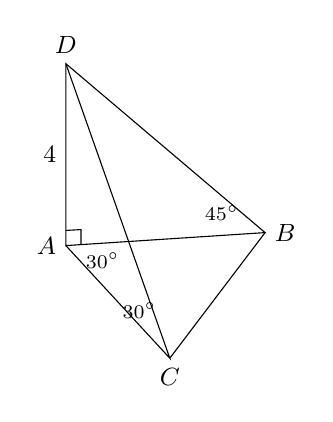
\begin{tikzpicture}[scale=0.55,font=\small]
\coordinate (A) at (0,0); \coordinate (D) at (0,4.2); \coordinate (B) at (4.6,0.3); \coordinate (C) at (2.4,-2.6);
\draw (D)--(A)--(B)--cycle; \draw (D)--(C)--(A); \draw (C)--(B);
\draw (0,0.35)--(0.35,0.37)--(0.35,0.02);
\node[left] at (A) {$A$}; \node[above] at (D) {$D$}; \node[right] at (B) {$B$}; \node[below] at (C) {$C$}; \node[left] at (0,2.1) {$4$};
\node at (3.6,0.75) {\scriptsize$45^\circ$}; \node at (0.85,-0.35) {\scriptsize$30^\circ$}; \node at (1.7,-1.5) {\scriptsize$30^\circ$};
\end{tikzpicture}}
\Opts{$6$}{$3$}{$2$}{$4$}}
\QQ{31}{$A=\{a,\ b,\ c,\ d,\ n,\ l\}$ va $B=\{a,\ b,\ k,\ d,\ m,\ n\}$ bölsa, $A\cap B$ ning böş bölmagan qism töplamlar sonini toping.
\Opts{$16$}{$15$}{$32$}{$31$}}
\QQ{32}{Raqamlari $6$ dan kiçik bölmagan uç xonali $3$ ga bölinadigan natural sonlar neçta?
\Opts{$18$}{$19$}{$20$}{$22$}}
\QQ{33}{\Moslash{Rasmda usti oçiq silindr va yarim şar tasvirlangan. ($\pi\approx3$)
\par\centering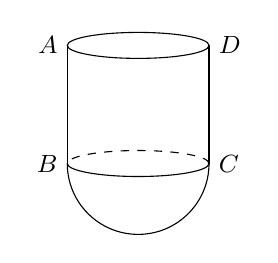
\begin{tikzpicture}[scale=0.75,font=\small]
\draw (0,2) ellipse (1.2 and 0.22); \draw (-1.2,2)--(-1.2,0); \draw (1.2,2)--(1.2,0);
\draw (-1.2,0) arc (180:360:1.2 and 0.22); \draw[dashed] (1.2,0) arc (0:180:1.2 and 0.22);
\draw (-1.2,0) arc (180:360:1.2);
\node[left] at (-1.2,2) {$A$}; \node[right] at (1.2,2) {$D$}; \node[left] at (-1.2,0) {$B$}; \node[right] at (1.2,0) {$C$};
\end{tikzpicture}}{A) $48$\par B) $32$\par C) $40$\par D) $30$\par E) $64$\par F) $70$}{Yarim şar hajmi silindr hajmiga teng. $AB=20$ cm bölsa, şar radiusini toping.}{$R=AB=2$ dm bölsa, jismning (idişning) töla sirtining yuzini toping.}{$R=AB=2$ dm bölsa, berilgan idişga neça litr suv ketadi?}}
\QQ{36}{$3x^2-4(3a-2)x+a^2+2a=0$ kvadrat tenglama berilgan.
\AB{Tenglama bitta ildizga ega böladigan $a$ ning barça qiymatlarining yiğindisini toping.}{Yeçimga ega bölmaydigan $a$ ning butun qiymatlari neçta?}}
\QQ{37}{$\sin x-\cos x+\sin3x=\cos3x+\cos5x-\sin5x$ tenglamani yeçing.
\AB{Tenglamaning $\left[-\dfrac\pi2;\,\pi\right]$ oraliğida yeçimlari neçta?}{Tenglamaning $\left[-\dfrac\pi2;\,\pi\right]$ kesmadagi barça yeçimlari yiğindisini toping.}}
\QQ{38}{$f(x)=x^3+ax+b$ ($a\ne b$) funksiyaga $x_0=a$, $x_0=b$ nuqtalarda ötkazilgan urinmalar parallel bölsa,
\AB{$f(1)$ ni hisoblang.}{$b=2$ bölsa $f'(1)$ ni hisoblang.}}
\QQ{39}{Funksiya grafigidan $f(2)=a$, $f(5)=b$ berilgan. $\displaystyle\int_2^5f(x)\cdot f'(x)\,dx=13{,}5$ va $a+b=9$ bölsa,
\qfig{\begin{tikzpicture}[x=0.65cm,y=0.45cm,font=\small]
\draw[-{Stealth[length=4pt]}] (-0.3,0)--(7,0) node[right] {$x$}; \draw[-{Stealth[length=4pt]}] (0,-0.3)--(0,6.6) node[left] {$y$};
\draw[thick] plot[smooth,tension=0.8] coordinates {(2,2.4) (2.15,3.1) (3,3.5) (4.2,4.0) (5,5) (5.5,6.2)};
\draw[dashed] (2,0)--(2,2.4)--(0,2.4); \draw[dashed] (5,0)--(5,5)--(0,5);
\node[below] at (2,0) {$2$}; \node[below] at (5,0) {$5$}; \node[left] at (0,2.4) {$a$}; \node[left] at (0,5) {$b$}; \node at (3.4,5.9) {$y=f(x)$};
\end{tikzpicture}}
\AB{$\dfrac{a-b}2$ ni hisoblang.}{$\displaystyle\int_2^5f(x)\,dx+\int_a^bf^{-1}(x)\,dx$ ni hisoblang ($f^{-1}(x)$ — $f(x)$ ning teskari funksiyasi).}}
\QQ{40}{$y=x^2$ parabolaga ikkita aylana urinagan ($A$ va $B$ nuqtalar) va ikkita aylana özaro urinagan ($C$ nuqtada).
\qfig{\begin{tikzpicture}[scale=0.95,font=\small]
\draw[-{Stealth[length=4pt]}] (-1.9,0)--(2,0) node[right] {$x$}; \draw[-{Stealth[length=4pt]}] (0,-0.2)--(0,4.6) node[left] {$y$};
\draw[thick,domain=-2.05:2.05,samples=60] plot (\x,{\x*\x}); \node[right] at (2.05,4.2) {$y=x^2$};
\draw (0,0.61) circle (0.6); \draw (0,2.81) circle (1.6);
\coordinate (A) at (0.332,0.11); \coordinate (B) at (1.52,2.31); \coordinate (O1) at (0,0.61); \coordinate (O2) at (0,2.81); \coordinate (C) at (0,1.21);
\draw[dashed] (O1)--(A); \draw[dashed] (O2)--(B); \draw[dashed] (0,0.11)--(A)--(0.332,0); \draw[dashed] (0,2.31)--(B)--(1.52,0);
\fill (A) circle (1.3pt); \fill (B) circle (1.3pt); \fill (O1) circle (1.3pt); \fill (O2) circle (1.3pt); \fill (C) circle (1.3pt);
\node[right] at (A) {$A$}; \node[right] at (B) {$B$}; \node[left] at (O1) {$O_1$}; \node[left] at (O2) {$O_2$}; \node[above left] at (C) {$C$};
\node[left] at (0,0.2) {\scriptsize$y_1$}; \node[left] at (0,2.31) {\scriptsize$y_2$}; \node[below left] at (0,0) {$O$}; \node[below] at (0.42,0) {\scriptsize$x_1$}; \node[below] at (1.52,0) {\scriptsize$x_2$};
\node[above] at (0.75,2.6) {$R$}; \node[above] at (0.2,0.42) {\scriptsize$r$};
\end{tikzpicture}}
\AB{$O_1$ va $(0;\,y_1)$ nuqtalar orasidagi masofani toping.}{$O_1A=r=2023$ bölsa, $O_2B$ ni toping.}}
\QQ{41}{$ABCD$ parallelogramm berilgan. $BH:BC=ED:AD=1:5$, \ $CG:BC=AL:AD=3:7$ bölsa,
\qfig{\begin{tikzpicture}[scale=0.62,font=\small]
\coordinate (A) at (0,0); \coordinate (D) at (7,0); \coordinate (B) at (3,4); \coordinate (C) at (10,4);
\coordinate (H) at (4.4,4); \coordinate (E) at (5.6,0); \coordinate (G) at (7,4); \coordinate (L) at (3,0); \coordinate (O) at (5,2);
\fill[qfill] (H)--(G)--(O)--cycle; \fill[qfill] (L)--(E)--(O)--cycle;
\draw (A)--(B)--(C)--(D)--cycle; \draw (H)--(E); \draw (L)--(G);
\node[below left] at (A) {$A$}; \node[above] at (B) {$B$}; \node[above right] at (C) {$C$}; \node[below right] at (D) {$D$};
\node[above] at (H) {$H$}; \node[above] at (G) {$G$}; \node[below] at (L) {$L$}; \node[below] at (E) {$E$}; \node[left] at (4.85,2.1) {$O$};
\end{tikzpicture}}
\AB{Böyalgan soha yuzining parallelogramm yuziga nisbatini toping.}{$ABHOL$ beşburçak yuzining parallelogramm yuziga nisbatini toping.}}
\QQ{42}{$ABC$ uçburçakka aylana içki çizilgan. $M$, $N$, $K$ nuqtalar aylananing $AB$, $AC$, $BC$ tomonlariga mos ravişda uriniş nuqtalari. Bunda $BK=3$, $KC=5$, $\angle ABC=60^\circ$ ga teng.
\qfig{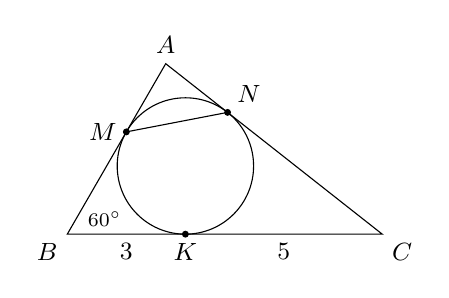
\begin{tikzpicture}[scale=0.5,font=\small]
\coordinate (B) at (0,0); \coordinate (C) at (8,0); \coordinate (A) at (2.5,4.33); \coordinate (I) at (3,1.732);
\coordinate (K) at (3,0); \coordinate (M) at (1.5,2.598); \coordinate (N) at (4.071,3.093);
\draw (A)--(B)--(C)--cycle; \draw (I) circle (1.732); \draw (M)--(N);
\fill (K) circle (2.5pt); \fill (M) circle (2.5pt); \fill (N) circle (2.5pt);
\node[above] at (A) {$A$}; \node[below left] at (B) {$B$}; \node[below right] at (C) {$C$}; \node[below] at (K) {$K$}; \node[left] at (M) {$M$}; \node[above right] at (N) {$N$};
\node[below] at (1.5,0) {$3$}; \node[below] at (5.5,0) {$5$}; \node at (0.95,0.38) {\scriptsize$60^\circ$};
\end{tikzpicture}}
\AB{$ABC$ uçburçakning yuzini toping.}{$MN$ kesmani toping.}}
\QQ{43}{$ABCDE$ beşburçak berilgan. $AB=BC=CD=DE$, $\angle B=96^\circ$, $\angle C=\angle D=108^\circ$ bölsa,
\qfig{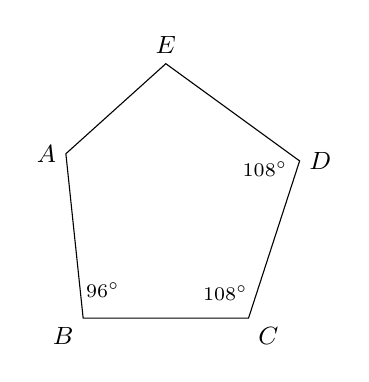
\begin{tikzpicture}[scale=2.1,font=\small]
\coordinate (B) at (0,0); \coordinate (C) at (1,0); \coordinate (D) at (1.309,0.951); \coordinate (E) at (0.5,1.539); \coordinate (A) at (-0.1045,0.9945);
\draw (A)--(B)--(C)--(D)--(E)--cycle;
\node[left] at (A) {$A$}; \node[below left] at (B) {$B$}; \node[below right] at (C) {$C$}; \node[right] at (D) {$D$}; \node[above] at (E) {$E$};
\node at (0.12,0.17) {\scriptsize$96^\circ$}; \node at (0.86,0.15) {\scriptsize$108^\circ$}; \node at (1.1,0.9) {\scriptsize$108^\circ$};
\end{tikzpicture}}
\AB{$\angle A$ ning içki burçagini toping.}{$\angle E$ ning içki burçagini toping.}}
\QQ{44}{Rasmda tasvirlangan şar va kub umumiy qismining (şarning kub içidagi qismi) hajmi şar hajmining $\dfrac1{12}$, kub hajmining esa $\dfrac1{16}$ qismini taşkil qiladi. Muntazam tetraedr va kub umumiy qismining (muntazam tetraedrning kub içidagi qismi) hajmi muntazam tetraedr hajmining $\dfrac1{10}$, kub hajmining esa $\dfrac1{20}$ qismini taşkil qiladi.
\qfig{\begin{tikzpicture}[scale=0.62,font=\small]
\draw (0,0) rectangle (3,3); \draw (0,3)--(1,3.8)--(4,3.8)--(3,3); \draw (4,3.8)--(4,0.8)--(3,0); \draw[dashed] (0,0)--(1,0.8)--(4,0.8); \draw[dashed] (1,0.8)--(1,3.8);
\fill[qfill] (0,1.5) ellipse (0.28 and 0.95); \draw (0,1.5) ellipse (0.28 and 0.95);
\draw (0,2.45) arc (75:285:0.98);
\coordinate (P1) at (3,1.3); \coordinate (P2) at (4.5,0.9); \coordinate (P3) at (5.4,1.6); \coordinate (P4) at (4.3,3.3);
\fill[qfill] (3,1.3)--(3.7,2.36)--(3.7,1.11)--cycle;
\draw (P1)--(P2)--(P3)--(P4)--cycle; \draw (P4)--(P2); \draw[dashed] (P1)--(P3);
\end{tikzpicture}}
\AB{Şar hajmining muntazam tetraedr hajmiga nisbatini toping.}{Agar muntazam tetraedrning qirrasi $6\sqrt2$ ga teng bölsa, kub hajmini toping.}}
\QQ{45}{Rasmda doiradan markaziy burçagi $\alpha$ ga teng bölgan sektor qirqib olindi. Qolgan qismidan konus yasaldi (böyalgan qism). ($\pi\approx3$, $\sqrt6\approx2{,}45$ deb oling.)
\qfig{\begin{tikzpicture}[scale=0.85,font=\small]
\fill[qfill] (0,0)--(60:1.5) arc (60:-240:1.5)--cycle; \draw (0,0) circle (1.5); \draw (60:1.5)--(0,0)--(120:1.5);
\draw (60:0.3) arc (60:120:0.3); \node at (90:0.5) {\scriptsize$\alpha$};
\begin{scope}[xshift=3.3cm,yshift=-1.3cm]
\fill[qfill] (-1.1,2.6)--(0,0)--(1.1,2.6) arc (0:-180:1.1 and 0.22);
\draw (0,2.6) ellipse (1.1 and 0.22); \draw (-1.1,2.6)--(0,0)--(1.1,2.6); \draw (0,0)--(0,2.6)--(1.1,2.6);
\draw (0,2.4)--(0.2,2.4)--(0.2,2.6);
\node[left] at (0,1.2) {$H$}; \node[right] at (0.6,1.3) {$R$};
\end{scope}
\end{tikzpicture}}
\AB{$\alpha=60^\circ$, $R=12$ ga teng bölsa, konus hajmini toping.}{Konus eng katta hajmga ega bölsa, $\alpha$ burçakni toping va butun qismigaça yaxlitlang.}}
\Javoblar{D B A B B A C C C D A B C C A A A A B A C C B A C A A B D D B D D A C}{%
\OK{36}{$\dfrac{18}{11}$}{$1$}\OK{37}{$7$}{$\dfrac{5\pi}3$}\OK{38}{$1$}{$1$}\OK{39}{$-\dfrac32$}{$24$}\OK{40}{$\dfrac12$}{$2024$}%
\OK{41}{$\dfrac{13}{70}$}{$\dfrac{57}{140}$}\OK{42}{$10\sqrt3$}{$\sqrt{\dfrac{48}7}$}\OK{43}{$126^\circ$}{$102^\circ$}\OK{44}{$\dfrac32$}{$144$}\OK{45}{$200\sqrt{11}$}{$66^\circ$}}
